\section{Alternative Methode: Random Forest}
\label{sec:Alternativ}
Das vorliegende binäre Klassifizierungsproblem wird über eine weitere Methode, den Random Forest gelöst.
Dieser kombiniert Ergebnisse mehrerer Entscheidungsbäume.
Die Entscheidungsbäume selbst werden zufällig und unkorreliert erstellt.
Jeder Baum trifft einzelne Entscheidungen, auf dessen Grundlage eine Finale Enscheidung gefällt wird.
\\
Folgende Features erhält der Random Forest als Eingabe:
\begin{itemize}
    \setlength\itemsep{0.1em}
    \item 3 Farbchannel und Graustufen
    \item Gradient für die 3 Farbchannel und der Graustufen
\end{itemize}
Ein Gradient gibt die Steigung bzw. Ableitung in einem Punkt an.
\begin{figure}
    \centering
    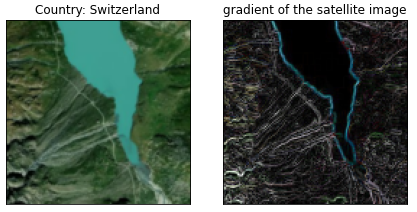
\includegraphics[width=0.6\textwidth]{content/img/gradient.png}
    \caption{Beispielhafte Darstellung des Gradienten der Farbchannel.\cite{mapbox}\cite{openstreetmap}}
    \label{fig:gradient}
\end{figure}
Hier beschreibt der Gradient die stärke der Farbänderung eines Pixels zu den benachbarten Pixeln.
Wie in \autoref{fig:gradient} zu sehen, können so Kanten detektiert werden.
\\
Aufgrund der hohen Auslastung des Arbeitsspeichers, wird der Random Forest auf $\SI{1000000}{}$ Pixel trainiert.
Die Pixel werden zufällig den Bildern des Trainingsdatensatzes entnommen.
Es ist nicht notwendig alle Pixel eines Bildes zu verwenden, da die Entscheidung Wasser/kein Wasser für jeden Pixel separat getroffen wird.
\\
Als maximale Tiefe der einzelnen Bäume hat sich $32$ und als Gesamtanzahl der Bäume $60$ durchgesetzt.
Die Ergebnisse werden auf der Metrik Genauigkeit evaluiert.
Obwohl der Random Forest mit gerade mal $\SI{1000000}{\text{px}}$ trainiert, ist auch hier kein Übertraining vorhanden.
Die Entscheidung ob in dem vorliegenden Pixel Wasser vorhanden ist, wird auschließlich über die Farbwerte und Gradienten bestimmt.
\FloatBarrier